%!TEX root = ../lections.tex
\subsection{Моды в линиях передачи}
Любая мода в лии передачи характеризуется поперечным волновым числом, а поперечное волновое число определяет продольное.

Так же у нас есть дисперсионное соотношение:
\begin{equation}
	h = \pm \sqrt{\frac{\omega^2}{c^2} \varepsilon \mu -\kappa^2_n}
\end{equation}

Можем ввести критическую длину волны:
\begin{gather}
	\kappa^2 = {\frac{\omega}{c}}^2 {\epsilon \mu}\\
	\omega_{cr} = \frac{\kappa c}{\sqrt{\epsilon \mu}}\\
	\lambda = \frac{2 \pi c}{\omega_{cr}} = \frac{2 \pi}{\kappa \sqrt{\epsilon \mu}}
\end{gather}

Если задана $\omega_{cr} / \lambda_{cr}$ можем говорить, распространяется данная волна или нет.

Если волна бежит вправо, то $h > 0$; если бежит влево, то $h < 0$

При  $\omega > \omega_{cr}$- режим распространяющейся волны.

\begin{equation}
	Re{\vec{E}} , Re{\vec{H}} \sim \cos(\omega t - h z)
\end{equation}

\begin{figure}[H]
	\centering
	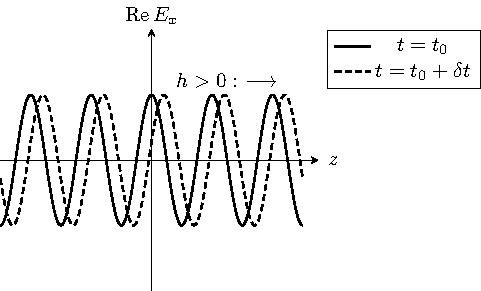
\includegraphics[scale=1.5]{img/lect3_ris1}
	\caption{Распространение волны ($h>0$)}
	\label{fig:lect3:1}
\end{figure}
При  $\omega < \omega_{cr}$- режим распространяющейся волны.

$h$ - мнимое.

\begin{equation}
	h = \pm i |h|
\end{equation}
\begin{equation}
	Re{E_x} \sim \cos(\omega t + \phi_0) \exp{\mp |h| z}
\end{equation}

Бегучести нет.

Зависимость экспонентальная
\begin{figure}[H]
	\centering
	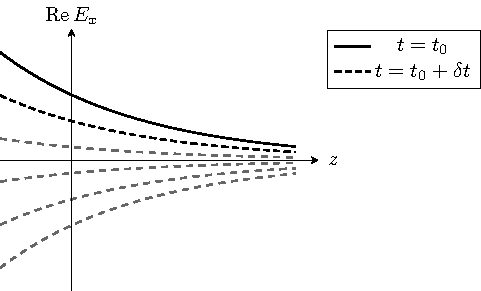
\includegraphics[scale=1.5]{img/lect3_ris2}
	\caption{Режим нераспространения ($h<0$)}
	\label{fig:lect3:2}
\end{figure}

\begin{figure}[H]
	\centering
	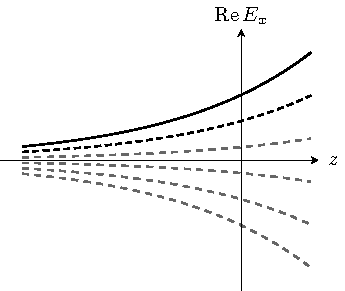
\includegraphics[scale=1.5]{img/lect3_ris3}
	\caption{Экспоненциальное нарастание амплитуды (при $h<0$)}
	\label{fig:lect3:3}
\end{figure}
Картинка зависит от способа создания волны, то есть у экспоненты " + или 		" - ". В зависимости от того, где источник можем сказать, куда бежит волна. То есть определить знак.

Источник может пораждать несколько мод, но не все, а какие-то конкретные.
\begin{figure}[H]
	\centering
	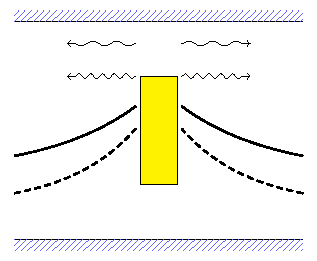
\includegraphics[scale=1.5]{img/lect3_ris4}
	\caption{Моды в линии передачи с источником}
	\label{fig:lect3:4}
\end{figure}
Изобразим числовую ось.
Пусть задана $\omega$, а то есть $k = \frac{\omega}{c} \sqrt{\epsilon \mu}$

Если $k < \kappa_1$ - все моды нераспространяющиеся.

Когда $k$ перейдёт через $\kappa_1$ появится низшая мода.

Когда перейдём через $\kappa_2$  появится ещё одна критическая частота.

!!Можно дополнить описание числовой прямой!!
\begin{figure}[H]
	\centering
	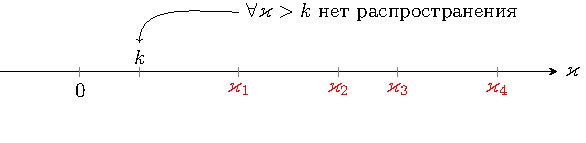
\includegraphics[scale=1.5]{img/lect3_ris5}
	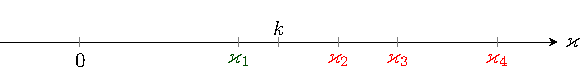
\includegraphics[scale=1.5]{img/lect3_ris6}
	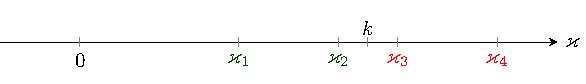
\includegraphics[scale=1.5]{img/lect3_ris7}
	% \label{fig:lect3:4}
\end{figure}

\subsection{Кинематические соотношения}
Определяют кинематические параметры волны.

\begin{enumerate}
	\item Временной период 

	\begin{equation}
		T = \frac{2 \pi}{\omega}
	\end{equation}

	\item Длина волны в волноводе (подразумевают линию передачи или трубу, когда говорят волновод)
	\begin{equation}
		\lambda_v = \frac{2 \pi}{h} = \frac{2 \pi}{\sqrt{k^2 - \kappa^2}} = \frac{2 \pi}{k} \frac{1}{\sqrt{1 - \frac{\kappa^2}{k^2}}} = \frac{\lambda_0}{\sqrt{1 - \frac{\omega_cr^2}{\omega}}} > \lambda_0
	\end{equation}

	Когда $\omega \rightarrow \omega_{cr}$	$\lambda_{v} \rightarrow \infty$

	$\lambda_0$ - длина волны в пространстве без волновoда в той же среде.

 	$\lambda_{v}$ - пространственный период.

 	\item Фазовая скорость - скорость перемещения плоскости постоянной фазы.

 	Поверхность постоянной фазы - это когда фаза константа.
 	\begin{equation}
 		faza = \omega t - h z + \phi_0
 	\end{equation}

 	При данном времени можно найти координату:
 	\begin{equation}
 		z = \frac{\omega t  + \phi_0}{ h }
 	\end{equation}

 	Координата будет перемещаться со скоростью:
 	\begin{equation}
 		v_f = \frac{\omega}{h}
 	\end{equation}
 	\begin{equation}
 		v_f = 
 		\frac{\omega}{\sqrt{k^2 - \kappa^2}} = 
 		\frac{\omega}{k} \frac{1}{\sqrt{1 - {\frac{k}{\kappa}^2}}} = \frac{\omega}{k} \frac{1}{\sqrt{1 - {\frac{\omega_{cr}}{\omega}^2}}} > v_f^{(0)}
	\end{equation}
	\begin{equation}
		v_f^{(0)} = \frac{c}{\varepsilon \mu} = \frac{\omega}{k}
	\end{equation}
 	Фазовая скорость может быть больше скорости света.

 	\item Групповая скорость - скорость перемещения квазимонохроматического волнового пакета. 

 	Волновой пакет - 

\begin{figure}[H]
	\centering
	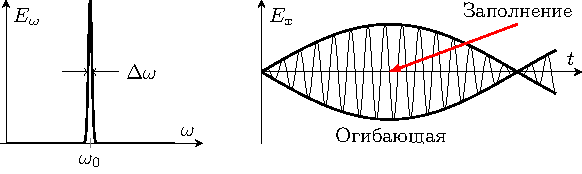
\includegraphics[scale=1.5]{img/lect3_ris8}
	\caption{Квазимонохроматический волновой пакет}
	\label{fig:lect3:8}
\end{figure}
	Сигнал характеризуется высокочастотным заполнением и огибающей.

\begin{figure}[H]
	\centering
	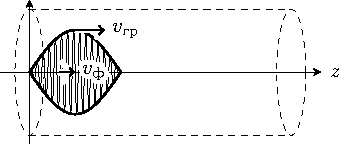
\includegraphics[scale=1.5]{img/lect3_ris9}
	\caption{Распространение волнового пакета}
	\label{fig:lect3:9}
\end{figure}
	По сути это радиоимпульс.

	Пакет движется со скоростью $ v_{gr} = \pdv{\omega}{k}\vert_{\omega = \omega_{0}} $ - это при малом или отсутствующем поглощении.(Это в пространстве, а не в линии передачи).

	При большом поглощении это понятие теряет смысл.

	По мере перемещения по волновду форма сигнала будет меняться.

	 $v_{gr} = \pdv{\omega}{h}\vert_{\omega = \omega_{0}} $ - формула для волновода. 

	 \begin{gather}
	 	k^2 = h^2 + \kappa^2\\
	 	%
	 	k = \frac{\omega}{c} \sqrt{ \varepsilon \mu}
	 \end{gather}

	Берём дифференциал от правой и левой части.$\kappa$  не зависит от частоты.
	\begin{gather}
		2k dk = 2h dh\\
		\pdv{\omega}{h} = \frac{c}{\sqrt{\varepsilon \mu}} \frac{h}{k}\\
		h = + \sqrt{\frac{\omega^2}{c^2} \varepsilon \mu -\kappa^2_n}\\
		\pdv{\omega}{h} = \frac{c}{\sqrt{\varepsilon \mu}} \frac{c}{\omega \sqrt{\varepsilon \mu}} \sqrt{\frac{\omega^2}{c^2} \varepsilon \mu -\kappa^2_n} = \frac{{v_f^{(0)}}^2}{v_f}
 	\end{gather}

 	\begin{gather}
 		v_{f} = \frac{\omega}{h}\\
 		v_{f}^{(0)} = \frac{c}{\omega \sqrt{\varepsilon \mu}}\\
 		%
 		v_{f} v_{gr} = {v_f^{(0)}}^2
 	\end{gather}
 	\begin{equation}
 		v_{gr} = v_{f}^{(0)} \sqrt{1 - {\frac{\omega_{cr}}{\omega}^2}}
 	\end{equation}

	Всё это справедливо для сред без временной дисперсии.
	\begin{equation}
		\varepsilon\ne f(\omega), \mu \ne f(\omega)
	\end{equation}

	!! есть ещё комментарии про дисперсию!!

	$v_{gr} < c$ - она несёт информацию.
\end{enumerate}
\begin{figure}[H]
	\centering
	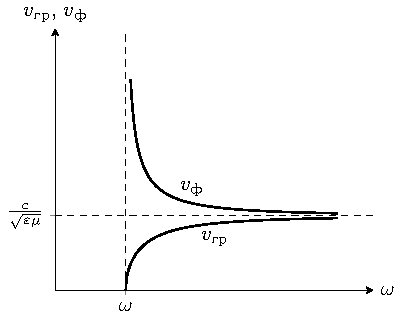
\includegraphics[scale=1.5]{img/lect3_ris10}
	\caption{Распространение волнового пакета}
	\label{fig:lect3:10}
\end{figure}

\subsection{Потоки энергии в линии передачи}
Когда идёт волна в линии передачи она переносит энергию.

Поток энергии характеризуется вектором Пойнтинга.

\begin{equation}
	\vec{S} = \frac{c}{4 \pi} [ Re{\vec{E}}, Re{\vec{H}}]
\end{equation}

Необходимо, чтобы уравнения были линейными
\begin{equation}
	Re{\vec{E}} Re{\vec{H}} \neq Re{(\vec{E} \vec{H})}
\end{equation}

Важная величина - среднее по времени.

Пусть есть
\begin{equation}
	A = A_0 \exp{i \omega t}
\end{equation}
\begin{equation}
	B = B_0 \exp{i \omega t}
\end{equation}
\begin{equation}
	\overline{Re{A}Re{B}} = \frac{1}{T} \int{Re{A}Re{B}}dt = \frac{1}{2} Re{A B*}
\end{equation}
где $\overline{A}$ - усреднение по времени, $B*$ - комплексно - сопряженное значение.
\begin{equation}
	\overline{\vec{S}} = \overline{\frac{4 \pi} [Re{\vec{E}}, Re{\vec{H}}]} = \frac{c}{8 \pi} Re[\vec{E}, \vec{H*}]
\end{equation}

 $\Sigma$ -  поперечное сечение линии передачи. 
Средний по времени поток:
\begin{equation}
	\Pi = \iint_{\Sigma} \overline{S_z} ds
\end{equation}
Поток - количество энергии, которое переносится через поперечное сечение за одну секунду.
$\overline{S_z}$ - проекция вектора Пойнтинга на ось z.
Вклад дают поперечные компоненты (в проекции на ось z).
\begin{equation}
	\overline{S_z} = \frac{c}{8 \pi} Re([\vec{E_\perp}, \vec{H*_\perp}], \vec{z_0})
\end{equation}
Можно переписать, если использовать соотношение:

\begin{equation}
	\vec{E_\perp} = \vartheta_{v \perp} [\vec{H_\perp}, \vec{z_0}]
\end{equation}
это в бегучей волне.

Подставив:
\begin{equation}
	\Pi = \frac{c}{8 \pi} Re{\vartheta_{v \perp}} \iint_{\Sigma} |\vec{H_\perp}|^2 ds
\end{equation}
или по-другому:
\begin{equation}
	\Pi = \frac{c}{8 \pi} 
		Re{\frac{1}{\vartheta_{v \perp})}} \iint_{\Sigma} |\vec{E_\perp}|^2 ds
\end{equation}
$\Pi$ ещё называют средней мощностью волны.
\begin{equation}
	\vartheta_{v \perp} = \sqrt{\frac{\mu}{\varepsilon}} {\frac{k}{h}}^{\pm 1}
\end{equation}
+ для ТЕ, - для ТМ.
$\omega < \omega_{kr}$- уравнение имеет только мнимые решения.
$h_n = 0$; 

Тогда $\vartheta_{v \perp}$  - мнимое, $Re$ часть равна нулю и поток энергии равен нулю.

$\omega > \omega_{kr}$ - мода имеет действительное h, волна распространяющаяся.
 $\vartheta_{v \perp}$- действительное, его реальная часть не равна нулю,поток энергии не равен нулю.
А что если в линии передачи несколько типов волн:

Пусть есть - $N$ мод.
\begin{equation}
	\Pi = \Sigma^{N}_{i = 1} \Pi_i
\end{equation}

Полный поток - сумма порциальных потоков.
Но здесь речь идёт о среднем.
